\documentclass{article}
\usepackage[bottom=2cm, right=1.5cm, left=1.5cm, top=2cm]{geometry}
\usepackage{amsmath}
\usepackage{amssymb}
\usepackage{amsthm}
\usepackage{enumitem}
\usepackage{exercise} % Exercises Style
\usepackage{graphicx}
\usepackage{caption}
\usepackage{environ}



% Enable Code
\usepackage{minted}
\let \extra T

\newcommand{\vect}[1]{\boldsymbol{\mathrm{#1}}}
\DeclareMathOperator{\tr}{tr}
\DeclareMathOperator{\Cov}{Cov}
\DeclareMathOperator{\Corr}{Corr}
\DeclareMathOperator{\Var}{Var}
\DeclareMathOperator{\E}{E}

\usepackage{fancyhdr}
\newenvironment{solution}
  {\renewcommand\qedsymbol{$\blacksquare$}\begin{proof}[Solution]$ $}
  {\end{proof}}

\title{Solutions to Assignment }
\author{Rongfei Jin}
\begin{document}

\pagestyle{fancy}
\fancyhf{}%
\fancyhead[L]{\textbf{ \ Assignment }}
\fancyhead[R]{\textbf{Rongfei Jin}}
\fancyfoot[C]{\thepage}%
\maketitle

\section*{Question 1}

We use the PACF to determine the order of the AR model. The PACF is defined as the correlation between $Y_t$ and $Y_{t-k}$ after removing the effect of all the intermediate variables $Y_{t-1}, Y_{t-2}, \ldots, Y_{t-(k-1)}$.

Consider the \(AR(p+1)\) model:
\begin{align*} 
Y_t &= a_0 + \sum_{k=1}^{p+1} a_k Y_{t-k} + \epsilon_t, \quad \epsilon_t
\end{align*}

Since the true model is \(AR(p)\), we have \(a_{p+1} = 0\) and the PACF should be zero for all lags greater than \(p\).

Now to determine the PACF, we can use the Yule-Walker equations, which relate the autocorrelations of the time series to the coefficients of the AR model and we can compute the significant levels to check if PACF is significantly different from zero.

See q1q2.py for the implementation.
\newpage
\section*{Question 2}

\begin{figure}[h!]
    \centering
    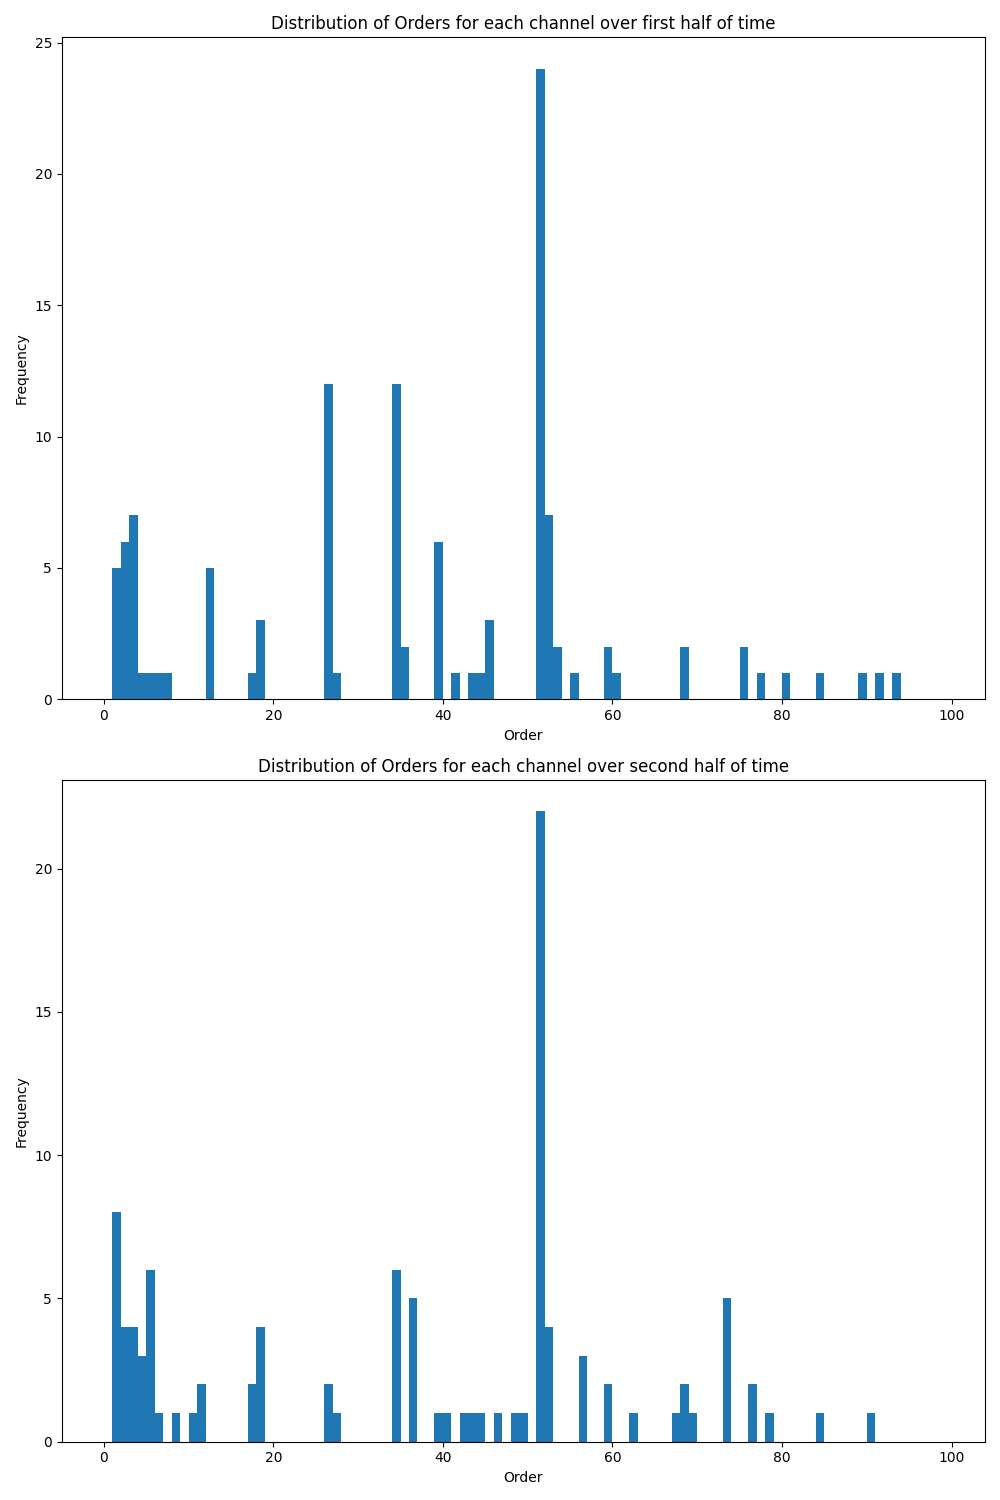
\includegraphics[width=0.6\textwidth]{figs/q2.png}
    \caption{Distribution of Orders for each channel over all time, first half of time, and second half of time}
    \label{fig:q2}
\end{figure}

We plot 4 histograms, the first one is the distribution of orders for each channel over all time, the second one is the distribution of orders for each channel over the first half of time, the third one is the distribution of orders for each channel over the second half of time, and the fourth one is the distribution of orders for each channel over the first half of time + 15 seconds.
We choose the onset time to be the first half of the data as we expect to see a different pattern between the two halves. The postictal data has more channels matching the AR order of 20, while the preictal data does not, this suggests that the epileptic activity changes the brain signal. We can also see some channels with greather than 20 orders when comparing the first half of time and the first half of time + 15 seconds, which may suggest the effect of the epileptic activity is not immediate.


\newpage
\section*{Question 3}
We first consdier the Autocovariance function
\[\gamma(h)  = \Cov(y_t, y_{t-h}) = \E[y_t y_{t-h}] - \E[y_t] \E[y_{t-h}]\]

and the correlation function
\[\Corr(y_t, y_{t-h}) = \frac{\Cov(y_t, y_{t-h})}{\sqrt{\Var(y_t) \Var(y_{t-h})}}\]

The ACF is defined as the correlation between $y_t$ and $y_{t-h}$ after removing the effect of all the intermediate variables $y_{t-1}, y_{t-2}, \ldots, y_{t-(h-1)}$. We express the ACF as
\[\rho(h) = \frac{\gamma(h)}{\gamma(0)}\]

The PACF is defined as the correlation between $y_t$ and $y_{t-h}$ after removing the effect of all the intermediate variables $y_{t-1}, y_{t-2}, \ldots, y_{t-(h-1)}$. We express the PACF for a staionary time series as
\[\phi_{11} = \gamma(1)\]
and 
\[\phi_{hh} = \Corr(y_{t+h} - \hat y_{t+h}, y_{t-h} - \hat y_{t-h})\]

where $\hat y_{t+h}$ and $\hat y_{t-h}$ are the predicted values of $y_{t+h}$ and $y_{t-h}$ using the regression model.

\[\hat y_{t+h} = \sum_{i=1}^{h-1} \beta_{i} y_{t + h - i }\]
\[\hat y_{t} = \sum_{i=1}^{h-1} \beta_{i} y_{t + i }\]

And the we can use the ACF and PACF to determine the order of the AR, MA, or ARMA model.
\begin{table}[!ht]
  \centering
  \begin{tabular}{|l|l|l|l|}
  \hline
      Function & AR(p) & MA(q) & ARMA(p,q) \\ \hline
      ACF & Tails off & Cuts off after lag q & Tails off \\ \hline
      PACF & Cuts off after lag p & Tails off & Tails off \\ \hline
  \end{tabular}
\end{table}

\section*{Question 4}

We first derive the ACF for MA(1) model.

\begin{align*}
  \gamma(1) &= \Cov(y_t, y_{t-1}) = \Cov(\epsilon_t - \theta_1 \epsilon_{t-1}, \epsilon_{t-1} - \theta_1 \epsilon_{t-2}) \\
  &= 0 + 0 + \theta_1 \sigma^2 + 0 = \theta_1 \sigma^2 \quad \epsilon_{k} \text{ are independent}
\end{align*}

\begin{align*}
  \gamma(0) &= \Var(y_t) = \Var(\epsilon_t - \theta_1 \epsilon_{t-1}) = \sigma^2 + \theta_1^2 \sigma^2 = (1 + \theta_1^2) \sigma^2
\end{align*}

\begin{align*}
  \rho(1) &= \frac{\gamma(1)}{\gamma(0)} = \frac{\theta_1 \sigma^2}{(1 + \theta_1^2) \sigma^2} = \frac{\theta_1}{1 + \theta_1^2}
\end{align*}

We estimate the ACF using the sample ACF, and we solve the equation for $\hat \theta_1$ 

\begin{align*}
  \hat \theta_1 &= \frac{1 \pm \sqrt{1 - 4 \hat \rho(1)^2}}{2 \hat \rho(1)}
\end{align*}

We then choose the solution $|\hat \theta_1| < 1$ for MA(1) model to be invertible, which is important for the equivalent AR model to be causal for further prediction.

See q4q5.py for the implementation.

\section*{Question 5}

The simulated data is actually MA(5) model, so both (i) and (ii) models are unable to capture the MA(5) model and produce a incorrect estimate of the parameters. By plotting the ACF and PACF, we can see that the ACF tails off and the PACF cuts off after lag 5, which is the order of the MA(5) model so with the proper order, we can estimate the parameters correctly.

See q4q5.py for the implementation.

\section*{Question 6}

We use auto-arima model to find the best model for each channel and plot the ACF and PACF of the residuals. And AR(3) models is the best model for most channels. We also notice that the the largest order of the AR model is 7 where the largest order of the MA model is 4. Based on our knowledge of the epileptic activity and brain signal, it is reasonable to infer that the brain signals have different frequency components. Since the data is collected from subject with epilepsy, we might expect the same pattern of the brain signal among other subjects.

\section*{Question 7}

Note that \(x_k, \vect{x_{-k}} \sim \mathcal{N}(\vect \mu, \vect \Theta^{-1})\), we can partition the mean and covariance matrix as

\begin{align*}
  \vect \mu &= \begin{pmatrix}
    \mu_k \\
    \vect \mu_{-k}
  \end{pmatrix}
\end{align*}

\begin{align*}
  \vect{\Theta} &= \begin{pmatrix}
    \vect \Theta_{kk} & \vect \Theta_{k,-k} \\
    \vect \Theta_{-k,k} & \vect \Theta_{-k,-k}
  \end{pmatrix}
\end{align*}

Notice that the kernel of the joint distribution of \(x_k\) and \(\vect{x_{-k}}\) is

\begin{align*}
\exp \left( - \frac{1}{2} (\vect x - \vect \mu)^T\Theta (\vect x - \vect \mu) \right)
\end{align*}

We can expand the quadratic form as

\begin{align*}
  (\vect x - \vect \mu)^T\Theta (\vect x - \vect \mu) &= \Theta_{kk}(x_k - \mu_k)^2 + 2 \Theta_{k,-k}(x_k - \mu_k)(\vect{x_{-k}} - \vect{\mu_{-k}}) + (\vect{x_{-k}} - \vect{\mu_{-k}})^T\Theta_{-k,-k}(\vect{x_{-k}} - \vect{\mu_{-k}})
\end{align*}

Now the conditional expectation of \(x_k\) given \(\vect{x_{-k}}\) is related to the \(x_k\) terms in the kernel of the joint distribution of \(x_k\) and \(\vect{x_{-k}}\). We can rewrite the terms in the kernel as

\[-\frac{1}{2} \left( {(x_k - \mu_k)^2}{\Theta_{kk}} + 2 {(x_k - \mu_k)(\vect{x_{-k}} - \vect{\mu_{-k}})}{\Theta_{k,-k}}   \right)\]

We can complete the square as

\begin{align*}
  -\frac{1}{2} \Theta_{kk}\left( (x_k - \mu_k + \frac{\Theta_{k,-k}}{\Theta_{kk}}(\vect{x_{-k}} - \vect{\mu_{-k}}))^2  \right)
\end{align*}

Based on the kernel, we can derive the conditional mean as 

\begin{align*}
  \E[x_k | \vect{x_{-k}}] &= \mu_k + \frac{\Theta_{k,-k}}{\Theta_{kk}}(\vect{x_{-k}} - \vect{\mu_{-k}})
\end{align*}

\section*{Question 8}
To estimate the \(\vect \Theta\), first notice that the previous expectation shows a linear relationship between \(x_k\) and \(\vect{x_{-k}}\). We can rewrite the expectation as

\begin{align*}
  \hat x_k &= \mu_k + \vect \beta^T(\vect{x_{-k}} - \vect{\mu_{-k}}) + \epsilon_k
\end{align*}

where \(\vect \beta = \frac{\Theta_{k,-k}}{\Theta_{kk}}\) and \(\epsilon_k \sim \mathcal{N}(0, \frac{1}{\Theta_{kk}})\).

Now we can use the lasso regression to estimate the \(\vect \Theta\) based on the linear relationship.

We let \(\hat \mu_k = x'_k\) and \(\hat{\vect{\mu}}_{-k} = \vect x'_{-k}\) where \(x'_k\) and \(\vect x'_{-k}\) are the sample data, we estimate the \(\frac{1}{\Theta_{kk}}\) as the inverse of the variance of the residuals.

\(\Theta_{kk} = \frac{\beta}{var(\epsilon_k)}\)

See q8.py for the implementation.

\section*{Question 9}

We first write the pdf of multivariate normal distribution as

\begin{align*}
  f(\vect x) = (2\pi)^{-\frac{n}{2}} \det(\vect \Sigma)^{-1/2} \exp\left(-\frac{1}{2} (\vect x - \vect \mu)^T\vect \Sigma^{-1}(\vect x - \vect \mu)\right)
\end{align*}

The log likelihood function is

\begin{align*}
  \log L(\vect \mu, \vect \Sigma) = -\frac{n}{2} \log(2\pi) - \frac{1}{2} \log(\det(\vect \Sigma)) - \frac{1}{2} (\vect x - \vect \mu)^T\vect \Sigma^{-1}(\vect x - \vect \mu)
\end{align*}

By using the determiant property, we can rewrite the log likelihood function as

\begin{align*}
  \log L(\vect \mu, \vect \Sigma) = -\frac{n}{2} \log(2\pi) + \frac{1}{2} \log(\det(\vect \Theta|)) - \frac{1}{2} (\vect x - \vect \mu)^T\vect \Sigma^{-1}(\vect x - \vect \mu)
\end{align*}

Notice that the last term is a scalar, so we can use associative properties of trace to rewrite the log likelihood function as

\begin{align*}
  \log L(\vect \mu, \vect \Theta) = -\frac{n}{2} \log(2\pi) + \frac{1}{2} \log(\det(\vect \Theta)) - \frac{1}{2} \tr(\vect S \vect \Theta)
\end{align*}

We now omit the constant term since we only consider the maximization with respect to \(\vect \Theta\).

\begin{align*}
  \log \det(\vect \Theta)- \vect S\vect \Theta
\end{align*}

Finally we can add the penalty term to the log likelihood function to get the penalized log likelihood function.

\begin{align*}
 \log \det(\vect \Theta)- \vect S\vect \Theta + \rho \|\vect \Theta\|_1
\end{align*}

\section*{Question 10}

The difference between the two methods is the first method is not based on the maximum likelihood estimator of the precision matrix, while the second method is and uses coordinate descent to estimate the precision matrix.

One advantage of the first method is that can be easily run in parallel, while the second method needs to compute the whole matrix. One limitation of the first method is that it may not produce a positive definite matrix. So a good senario for the first method is when the sample size is large and the sample precision matrix is close to the true precision matrix.

See q10.py for the implementation.

\section*{Question 11}




















\end{document}
% To estimate the $AR(p)$ model, we can use Maximal Likelihood Estimation (MLE). 
% First we notice that the conditional distribution of $Y_t$ given the past values is Gaussian since the only random variable in the model is $\epsilon$ itself. The model can be written as:

% \[Y_t | y_{t-1}, \ldots, y_{t-k} \sim N(a_0 + \sum_{k=1}^{p} a_k y_{t-k}, \sigma^2)\]

% then the conditional density function is:
% \begin{align*}
% f(Y_t = y_t | y_{t-1}, \ldots, y_{t-p}) &= \frac{1}{\sqrt{2\pi\sigma^2}} \exp\left(-\frac{(y_t - (a_0 + \sum_{k=1}^{p} a_k y_{t-k}))^2}{2\sigma^2}\right)\\
% \end{align*}

% The likelihood function for the entire sample is the product of the conditional densities:

% \begin{align*}
% L(a_0, a_1, \ldots, a_p, \sigma^2) &= \prod_{t=p+1}^{n} f(Y_t = y_t | y_{t-1}, \ldots, y_{t-p})\\
% &= \prod_{t=p+1}^{n} \frac{1}{\sqrt{2\pi\sigma^2}} \exp\left(-\frac{(y_t - (a_0 + \sum_{k=1}^{p} a_k y_{t-k}))^2}{2\sigma^2}\right)\\
% &= \left(\frac{1}{\sqrt{2\pi\sigma^2}}\right)^{n-p} \exp\left(-\frac{1}{2\sigma^2} \sum_{t=p+1}^{n} (y_t - (a_0 + \sum_{k=1}^{p} a_k y_{t-k}))^2\right)
% \end{align*}

% To find the MLE, we take the logarithm of the likelihood function:
% \begin{align*}
% \log L(a_0, a_1, \ldots, a_p, \sigma^2) &= -\frac{n-p}{2} \log(2\pi) - \frac{(n-p)}{2} \log(\sigma^2) - \frac{1}{2\sigma^2} \sum_{t=p+1}^{n} (y_t - (a_0 + \sum_{k=1}^{p} a_k y_{t-k}))^2
% \end{align*}
